\subsection{Additional Centralities}\label{additional-centralities}

\subsubsection{The \emph{Gravity Index}}

The \emph{Gravity Index} uses spatial impedance to measure accessibility, emphasising potential interaction flows over the street network \cite{Batty2013, Hansen1959, Rutherford1979}. Like gravitational attraction, the measure reflects how interaction potential decays with distance, typically through the negative exponential
\begin{equation}\label{eq:gravity}
  Gravity_{(i)}=\sum_{j\neq{i}}\exp(-\beta\cdot d)
\end{equation}
where the rate of decay $\beta$ (in the negative exponential) can be set to model specific trip-purposes or transportation modes to reflect people's willingness to travel a given distance $d$ to particular types of locations \cite{Sevtsuk2012, Handy1997, Iacono2008}. A variety of different impedance functions can be used, though these tend to behave similarly \cite{vale_influence_2017}.

The term \emph{Gravity Index} is potentially misleading. Full gravity models account for the attraction of origins and destinations, whereas the \emph{Gravity Index} assumes equal attraction from each node to every other node. It provides distance-weighted counts of accessible locations $j$ proximate to $i$ at a given impedance $\beta$---useful for quantifying access to specific land-uses or, for street network structure, physical accessibility. Varying the decay parameter emphasises smaller or larger network structures.

\begin{figure}[htp]
  \centering
  \includegraphics[width=\linewidth, keepaspectratio]{images/gravity_decay.pdf}
  \caption{Spatial impedance curves for different $\beta$ parameters. Nearer locations can be weighted more heavily than farther locations through use of the negative exponential decay function.}\label{fig:beta_decays}
\end{figure}

Gravity measures are inherently localised and do not strictly require distance cutoffs, though computational efficiency favours thresholds where decay renders additional computation negligible (Figure~\ref{fig:beta_decays}). Here, $\beta$ parameters are anchored to distance thresholds $d_{max}$ through $\beta = 4 / d_{max}$. For example, $d_{max}=100m$ corresponds to $\beta=0.04$ and an average trip distance of $35m$. These impedances are calibrated for pedestrians: $\beta=0.005$ ($d_{\max}=800m$) represents typical walking distances to bus stops \cite{Sevtsuk2016, Handy1997}. Willingness to walk varies by trip purpose---pedestrians walk farther for recreation than shopping \cite{Iacono2008}---and by location, with North American contexts less supportive of walking than European equivalents \cite{Reyer2014}. Generally, pedestrians are unwilling to walk more than a mile ($1600m$, $\beta\approx0.0025$) for non-recreational purposes, and exponential decay reflects the preference for nearer destinations \cite{Baradaran2001, Scheurer2007, Duncan2011, Handy2001, Harris2001, Bates2007}.

\subsubsection{Betweenness centrality}

Unless nodes $j$ and $k$ are directly adjacent, shortest paths between them pass through intermediate nodes $i$. \emph{Betweenness}
\begin{equation}\label{eq:betweenness}
  Betweenness_{(i)} = \sum_{j\neq{i}} \sum_{k\neq{j}\neq{i}} n(j, k)\ i
\end{equation}
is the sum of shortest paths between all $(j, k)$ node pairs passing through node $i$ \cite{Freeman1977}. For street networks, it conveys how likely a street is to be traversed by people travelling between other locations. The Space Syntax community refers to this measure as \emph{Choice}. Localised \emph{Betweenness} considers only $(j, k)$ pairs within threshold cutoff distances.

\emph{Betweenness} can be weighted by distances:
\begin{equation}\label{eq:weighted_betweenness}
  Betweenness_{(i)}=\sum_{j\neq{i}}\sum_{k\neq{j}\neq{i}} n(j, k)\ i\cdot\exp(-\beta\cdot d)\, ,
\end{equation}
in which case the negative exponential (see~\ref{eq:gravity}) can be used to reflect the notion that trips between closely located $(j, k)$ node-pairs are more likely to occur than those located farther apart, with $d$ in this case representing the corresponding trip distance for a given $(j, k)$ pair of nodes passing through node $i$.

Space Syntax methods also include normalised least angular choice \emph{(NACH)}, described as a normalised form of \emph{Betweenness} (Choice) achieved through division by \emph{Farness} (Total Depth)
\begin{equation}\label{eq:nach}
  NACH{(i)}=\frac{\log(Betweenness + 1)}{\log(Farness + 3)}.
\end{equation}
This is more accurately described as a hybrid measure---a betweenness-weighted closeness measure---rather than a normalisation. The originators state that \emph{``it seems to combine our two measures -- depth and choice, to and through-movement''} \cite{Hillier2012}. The constants in numerator and denominator guard against taking the logarithm of values less than 1.

\subsubsection{Length-weighting}
Varying node intensities can distort centrality measures. Weighting nodes by street lengths \cite{Turner2005a, Turner2007} or adjacent building counts \cite{Sevtsuk2012} addresses this: greater exposure to street length implies greater interaction potential, while high node concentrations are tempered by correspondingly shorter segments. In the dual representation, primal street segment lengths are assigned to dual nodes and incorporated into the centrality calculation. For \emph{Harmonic Closeness}, the $1$ in the numerator is replaced by segment length $l$:
\begin{equation}\label{eq:harmonic_length_weighted}
  HC_{(i)} = \sum_{j\neq{i}}\frac{l}{d_{(i,j)}}\, .
\end{equation}

An alternative uses the integral of \emph{Harmonic Closeness}. The integral for $f(x)=1/d$ takes the form
\begin{equation}
  \int_{a}^{b}\ f(x)\ dx = \ln(b) - \ln(a)
\end{equation}
and can be applied to sum the `area under the (spatial impedance) curve' for the respective lower and upper segment bounds $a$ and $b$ for all reachable segments $S$:
\begin{equation}\label{eq:harmonic_integral}
  HC_{(i)} = \sum_{(a, b)}^{S} \int_{a}^{b}\ f(x)\ dx = \sum_{(a, b)}^{S}\ \ln(b) - \ln(a)\, .
\end{equation}
This allows spatial impedances to increase continuously. For example, the contribution of a 10m street segment adjacent to the origin is now found as $\ln(10) = 2.303$ and a segment from $10m$ to $20m$ distant is found as $\ln(20) - \ln(10) = 0.693$. As shown in Figure~\ref{fig:closeness_comparisons_length_weighted} and Table~\ref{table:closeness_comparisons_length_weighted}, the continuous form remains consistent regardless of how many times street lengths are split at intervening nodes.

\begin{figure}[htp]
  \centering
  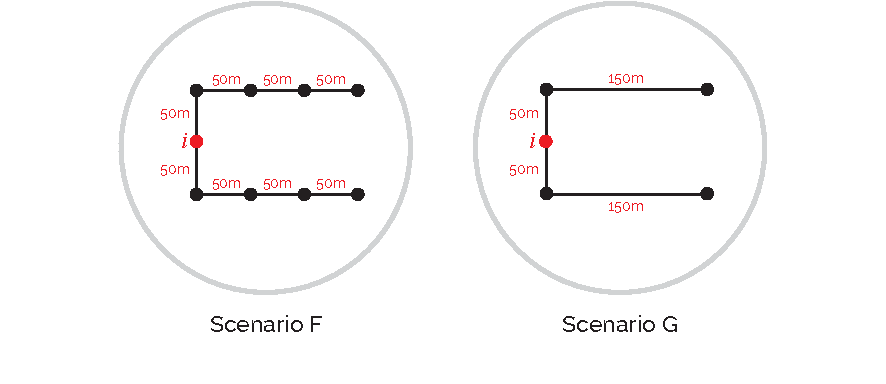
\includegraphics[width=\linewidth, keepaspectratio]{images/closeness_comparisons_length_weighted.pdf}
  \caption{Length weighted closeness formulations comparing for varied node intensities.}\label{fig:closeness_comparisons_length_weighted}
\end{figure}

\begin{table*}[htp]
  \centering
  \begin{tabular}{ r | r r }
    &
    $length\ wt.\ HC_{(i)} = \sum_{j\neq{i}}\frac{l}{d_{(i,j)}}$ &
    $Harmonic\ C_{(i)} (0, x) = \int_{0}^{x} \ln(x)\ dx$ \\
    \midrule
    \\
    Scenario F &
    $(\frac{50}{50} + \frac{50}{100} + \frac{50}{150} + \frac{25}{200})*2 = 3.92$ &
    $(simplified)\ \ln(200) * 2 = 10.60$ \\
    \\
    Scenario G &
    $(\frac{100}{50} + \frac{75}{200})*2 = 4.75$ &
    $(simplified)\  \ln(200) * 2 = 10.60$ \\
  \end{tabular}
  \caption{Length weighted closeness formulations comparing street-length weighted \emph{Harmonic Closeness} and a continuous form of \emph{Harmonic Closeness}. Continuous forms remain consistent regardless of the number of subdivisions.}\label{table:closeness_comparisons_length_weighted}
\end{table*}

The continuous form of \emph{Harmonic Closeness} (Equation~\ref{eq:harmonic_integral}) cannot be used with \emph{geometric distance} (angular) impedances, which do not increase continuously.

The gravity index can also be expressed in continuous form, computed as the area under the curve for all reachable segments $S$ with lower and upper bounds $a$ and $b$ at impedance $\beta$:
\begin{equation}\label{eq:gravity_continuous}
  G_{(i)} = \sum_{(a, b)}^{S} \int_{a}^{b}\ f(x)\ dx = \sum_{(a, b)}^{S}\ \frac{\exp(-\beta\cdot b) -\exp(-\beta\cdot a)}{-\beta}.
\end{equation}